\section{Расчет второго вириального коэффициента и квантовых поправок}

\subsection{Групповое разложение \cite{eremin, hirsch}}

Рассмотрим однокомпонентный классический газ, состоящий из $N$ одинаковых частиц и занимающих объем $V$. Предположим, что парные взаимодействия частиц являются центральными, и общая потенциальная энергия $U$ является суммой парных взаимодействий частиц $u = u(r)$. В таком случае полная потенциальная энергия системы может быть записана в виде $U \lb \mathbf{r}^N \rb = \displaystyle \dfrac{1}{2} \sum_{i, j} u_{ij}$, где $u_{ij}$ -- потенциал взаимодействия для изолированной пары молекул (Это предположение справедливо, за исключением случаев молекул, имеющих тенденцию к ассоциированию.). Конфигурационный интеграл газа $Z_N$ запишется в виде:
\vverh
\begin{gather}
	Z_N (T, V) = \int_V \cdots \int_V \exp \lb - \frac{\displaystyle\sum_{1 \leqslant i < j \leqslant N} u \lb r_{ij} \rb}{kT} \rb d \mathbf{r}_1 d \mathbf{r}_2 \dots \mathbf{r}_N = \notag \\
	= \int_V \cdots \int_V \prod_{1 \leqslant i < j \leqslant N} \exp \lb - \frac{u \lb r_{ij} \rb}{KT} \rb d \mathbf{r}_1 d \mathbf{r}_2 \dots d \mathbf{r}_N \label{confint}
\end{gather}

Функция Майера определена соотношением
\vverh
\begin{gather}
	\exp \lb - \frac{u \lb r_{ij} \rb}{kT} \rb = 1 + f_{ij} . \label{mayer}
\end{gather}
Функция $f = f(r)$ обладает следующими общими свойствами в зависимости от расстояния: при $r \longrightarrow 0: f(r) \longrightarrow -1$, затем $f(r)$ монотонно возрастает, проходит через максимум при расстоянии $r = d_0$, отвечающему минимуму потенциала $u(r)$, и при дальнейшем увеличении растояния между частицами она монотонно убывает, $f(r) \longrightarrow 0$ при $r \longrightarrow \infty$, оставаясь положительной. Таким образом, функция Майера существенно отлична от нуля только при расстояниях, отвечающих достаточно близкому расположению частиц. Подставляя выражение \eqref{mayer} в выражение для конфигурационного интеграла \eqref{confint}, получаем
\vverh
\begin{gather}
	Z_N (T, V) = \int_V \cdots \int_V \prod_{1 \leqslant i < j \leqslant N} \lb 1 + f_{ij} \rb d \mathbf{r}_1 d \mathbf{r}_2 \dots d \mathbf{r}_N , \label{confint1}
\end{gather}
в которой подынтегральное выражение есть произведение $\displaystyle\frac{N \lb N - 1 \rb}{2}$ функций $\lb 1 + f_{ij} \rb$, каждая из которых соответсвует определенной паре частиц. Раскрывая произведение в \eqref{confint1}, получаем
\vverh
\begin{gather}
	Z_N = \int_V \cdots \int_V \lb 1 + \sum_{i < j} f_{ij} + \sum_{i, j} \sum_{k,l} f_{ij} f_{kl} + \dots \rb d \mathbf{r}_1 d \mathbf{r}_2 \dots d \mathbf{r}_N = \int_V \cdots \int_V d \mathbf{r}_1 d \mathbf{r}_2 \dots d \mathbf{r}_N + \notag \\ 
	+ \sum_{i < j} \int_V \cdots \int_V f_{ij} d \mathbf{r}_1 d \mathbf{r}_2 \dots d \mathbf{r}_N + \sum_{i, j} \sum_{k, l} \int_V \cdots \int_V f_{ij} f_{kl} d \mathbf{r}_1 d \mathbf{r}_2 \dots d \mathbf{r}_N + \dots \label{confint2}  
\end{gather}

\subsection{$N$-частичные графы \cite{mayer}}
Каждому члену в разложении \eqref{confint2} можно сопоставить $N$-частичный граф, состоящий из $N$ пронумерованных вершин, соединенных ребрами в том случае, если в подынтегральном выражении функция Майера, содержащая индексы рассматриваемых вершин.

\begin{figure}[!ht]
\centering
\begin{minipage}{0.3\linewidth}
	\begin{tikzpicture}
	[vertex/.style={circle, draw=blue!50, fill=blue!20, thick}]
	\node[vertex] (1) {1};
	\node[vertex] (2) [below = 1cm of 1] {2}
		edge [thick] (1);
	\node[vertex] (3) [right = 1cm of 1] {3};
	\node[vertex] (4) [below = 1cm of 3] {4};
	\node[vertex] (5) [right = 1cm of 3] {5}
		edge [thick] (4);
	\node[vertex] (6) [below = 1 cm of 5] {6}
		edge [thick] (5);
	\begin{scope}[on background layer]
		\node [fill=yellow!20,fit=(1) (2) (5) (6)] {};
	\end{scope}
	\end{tikzpicture}
\end{minipage}%
\begin{minipage}{0.5\linewidth}
		\begin{equation*}
			\int \cdots \int f_{12} f_{45} f_{56} \, d \mathbf{r}_1 d \mathbf{r}_2 \dots d \mathbf{r}_6
		\end{equation*}
\end{minipage}
\caption{Пример $6$-частичного интеграла и соответствующего графа. }
\end{figure}

Назовем $l$-группой такой $l$-частичный граф, в котором к каждой вершине подходит по крайней мере одно ребро ($l$-группа -- связный $l$-частичный граф). Очевидно
\vverh
\begin{gather}
	\sum_l l m_l = N \label{cond1}
\end{gather}
Обозначим через $m_l$ число $l$-групп для данного $N$-частичного графа, являющегося членом разложения конфигурационного интеграла $Z_N$. Данному набор чисел $\left\{ m_l \right\} = \left\{ m_1 , m_2 , \dots, m_N \right\}$, $( m_l \geqslant 0 )$ отвечает некоторая совокупность $N$-графов, сумму которых обозначим через $S_N \left( \left\{ m_l \right\} \right)$, тогда:
\vverh
\begin{gather}
	Z_N = \sum_{ \left\{ m_l \right\} } S_N \left( \left\{ m_l \right\} \right), \label{confsum}
\end{gather}
где суммирование проводится по всем наборам чисел $\left\{ m_l \right\}$, удовлетворяющих условию \eqref{cond1}. \par
Диаграммы, образующие $S_N \left( \left\{ m_l \right\} \right)$, отличаются, во-первых, способом распределения пронумерованных частиц по группам. Во-вторых, $l$-группы при $l \geqslant 3$ могут быть составлены из данных пронумерованных частиц различными способами. Так, при $N=4$, $m_1 = 1$, $m_2 = 0$, $m_3 = 1$, при распределении пронумерованных частиц $1; 2-3-4$ будут различными следующие четыре диаграммы:
\vverh
\begin{figure}[h]
	\begin{minipage}{0.33\linewidth}
		\begin{tikzpicture}
			[vertex/.style={circle, draw=blue!50, fill=blue!20, thick}]
			\node (dummy) {};
			\node[vertex] (1) [below = -0.1cm of dummy] {1};
			\node[vertex] (2) [below right = 1cm and 1.3cm of dummy] {2};
			\node[vertex] (3) [above right = 1cm and 0.6cm of 2] {3}
				edge [thick] (2); 
			\node[vertex] (4) [below right = 1cm and 0.6cm of 3] {4}
				edge [thick] (3);
			\begin{scope}[on background layer]
				\node [fill=yellow!20,fit=(1) (2) (3) (4)] {};
			\end{scope}
		\end{tikzpicture}
		\caption*{$\displaystyle\int d \mathbf{r}_1 \int \int \int f_{23} f_{34} \, d \mathbf{r}_2 d \mathbf{r}_3 d \mathbf{r}_4$}
	\end{minipage}
	\begin{minipage}{0.33\linewidth}
		\begin{tikzpicture}
			[vertex/.style={circle, draw=blue!50, fill=blue!20, thick}]
			\node (dummy) {};
			\node[vertex] (1) [below = -0.1cm of dummy] {1};
			\node[vertex] (2) [below right = 1cm and 1.3cm of dummy] {2};
			\node[vertex] (3) [above right = 1cm and 0.6cm of 2] {3}
				edge [thick] (2); 
			\node[vertex] (4) [below right = 1cm and 0.6cm of 3] {4}
				edge [thick] (2);
			\begin{scope}[on background layer]
				\node [fill=yellow!20,fit=(1) (2) (3) (4)] {};
			\end{scope}
		\end{tikzpicture}
		\caption*{$\displaystyle \int d \mathbf{r}_1 \int \int \int f_{23} f_{24} \, d \mathbf{r}_2 d \mathbf{r}_3 d \mathbf{r}_4$}
	\end{minipage}
	\begin{minipage}{0.33\linewidth}
		\begin{tikzpicture}
			[vertex/.style={circle, draw=blue!50, fill=blue!20, thick}]
			\node (dummy) {};
			\node[vertex] (1) [below = -0.1cm of dummy] {1};
			\node[vertex] (2) [below right = 1cm and 1.3cm of dummy] {2};
			\node[vertex] (3) [above right = 1cm and 0.6cm of 2] {3};
			\node[vertex] (4) [below right = 1cm and 0.6cm of 3] {4}
				edge [thick] (3)
				edge [thick] (2);
			\begin{scope}[on background layer]
				\node [fill=yellow!20,fit=(1) (2) (3) (4)] {};
			\end{scope}
		\end{tikzpicture}
		\caption*{$\displaystyle \int d \mathbf{r}_1 \int \int \int f_{24} f_{34} \, d \mathbf{r}_2 d \mathbf{r}_3 d \mathbf{r}_4$}
	\end{minipage} \\
	\begin{center}
	\begin{minipage}{0.33\linewidth}
		\begin{tikzpicture}
			[vertex/.style={circle, draw=blue!50, fill=blue!20, thick}]
			\node (dummy) {};
			\node[vertex] (1) [below = -0.1cm of dummy] {1};
			\node[vertex] (2) [below right = 1cm and 1.3cm of dummy] {2};
			\node[vertex] (3) [above right = 1cm and 0.6cm of 2] {3}
				edge [thick] (2);
			\node[vertex] (4) [below right = 1cm and 0.6cm of 3] {4}
				edge [thick] (3)
				edge [thick] (2);
			\begin{scope}[on background layer]
				\node [fill=yellow!20,fit=(1) (2) (3) (4)] {};
			\end{scope}
		\end{tikzpicture}
		\caption*{$\displaystyle \int d \mathbf{r}_1 \int \int \int f_{23} f_{24} f_{34} \, d \mathbf{r}_2 d \mathbf{r}_3 d \mathbf{r}_4$}
	\end{minipage}
\end{center}
\caption{Четыре варианта $3$-групп при $N = 4$ и фиксированном распределении $ \left\{ \left\{ 1 \right\}, \left\{ 2, 3, 4 \right\} \right\}$ с соответствующими интегралами.}
\end{figure}

Члены разложения, в которых одни и те же молекулы связаны друг с другом в групп, обладают тем общим свойством, что они отличны от нуля лишь в той области конфигурационного пространства, в которой молекулы одной группы находятся близко друг к другу.

Если число $l$-групп равно $m_l$, то они дают сомножитель, дающий вклад в $S_N \lb \left\{ m_l \right\} \rb$, который будем обозначать $\bigg[ \text{сумма всех $l$-групп} \bigg]^m_l$, называемый групповой функцией (\textit{cluster function} \cite{mayer}). Так 3-группы дают сомножитель
\vverh
\begin{gather}
\int d \mathbf{r}_1 \int \int \int f_{23} f_{34} \, d \mathbf{r}_2 d \mathbf{r}_3 d \mathbf{r}_4 + $ $+ \displaystyle \int d \mathbf{r}_1 \int \int \int f_{23} f_{24} \, d \mathbf{r}_2 d \mathbf{r}_3 d \mathbf{r}_4 + \int d \mathbf{r}_1 \int \int \int f_{24} f_{34} \, d \mathbf{r}_2 d \mathbf{r}_3 d \mathbf{r}_4 + \notag \\ + \int d \mathbf{r}_1 \int \int \int f_{23} f_{24} f_{34} \, d \mathbf{r}_2 d \mathbf{r}_3 d \mathbf{r}_4. \notag
\end{gather}
Для оценки суммы $S_N \left( \left\{ m_l \right\} \right)$ необходимо найти число способов распределения $N$ частиц на $l$-групп так, чтобы число $l$-групп равноялось $m_l$ ($l = 1, 2 \dots N$). Из комбинаторных соображений искомое число способов равно
\vverh
\begin{gather}
	\dfrac{N!}{\displaystyle\prod_{l=1}^{N} \left( l! \right)^{m_l} \cdot m_l !} \notag 
\end{gather}

В итоге получаем следующий вид суммы $S_N \left( \left\{ m_l \right\} \right)$:
\vverh
\begin{gather}
	S_N \left( \left\{ m_l \right\} \right) = \dfrac{N!}{\displaystyle \left( l! \right)^{m_l} \cdot m_l!} \prod_{l} \bigg[ \text{сумма всех $l$-групп} \bigg]^m_l \label{snexp}
\end{gather}

\subsection{Групповые интегралы \cite{mayer}}

Групповые интегралы $b_l$ вводятся посредством следующих выражений:
\vverh
\begin{gather}
	b_{\, l} = \frac{1}{l! V} \bigg[ \text{сумма всех $l$-групп} \bigg]^m_l . \label{groupint}
\end{gather}

Рассмотрим первые групповые интегралы:
\vverh
\begin{gather}
	b_1 = \frac{1}{V} \int_V d \mathbf{r}_1 = 1, \notag \\
	b_2 = \frac{1}{2 V} \int_V \int_V f \lb r_{12} \rb \, d \mathbf{r}_1 d \mathbf{r}_2 = \frac{1}{2} \int_V f \lb r \rb d \mathbf{r} = - 2 \pi \int_{0}^{\infty} \lb 1 - \exp \lb - \frac{u \lb r \rb}{kT} \rb r^2 d r \label{b2int}  
\end{gather}

Т.к. $f_{ij}$ зависит только от расстояния между частицами $r_{ij}$, но не от положения группы, то интегрирование можно выполнить в два шага: сначала по координатам одной из частиц, что дает множитель $V$, и перейти к относительным координатам для всех остальных частиц групп, что и сделано в преобразованиях $b_2$ \eqref{b2int}. При дальнейшим преобразовании $b_2$ в \eqref{b2int} введены сферические координаты для второй частицы, $r, \varphi, \theta$, интегрирование по сферическим перменным дает множитель $4 \pi$. Выбор в качестве верхнего предела интегрирования за бесконечность предполагает, что частицы находятся вдалеке от стенок, и в силу быстрого убывания $f(r)$ нет необходимости учитывать геометрические параметры сосуда. Поэтому групповые интегралы не зависят от объема системы и являются функциями только температуры.  

Используем определение групповых интегралов \eqref{groupint} в выражении \eqref{snexp}:
\vverh
\begin{gather}
	S_N \lb \left\{ m_l \right\} \rb = \frac{N!}{\displaystyle\prod_{l=1}^{N} \lb l! \rb^{m_l} \cdot m_l !} \prod \lb b_l l! V \rb^{m_l} = N! \prod_l \frac{1}{m_l!} \lb V b_l \rb^{m_l} \label{snexp2}
\end{gather}

Используя полученный результат в выражении \eqref{confsum} для конфигурационного интеграла $Z_N$, получаем
\vverh
\begin{gather}
	Z_N = \sum_{\left\{ m_l \right\}} S_N \lb \left\{ m_l \right\} \rb = N! \sum_{\left\{ m_l \right\}} \prod_l \frac{1}{m_l!} \lb V b_l \rb^{m_l}. \label{confsum2}
\end{gather}

\subsection{Связь вириальных коэффициентов и групповых интегралов \cite{mayer, meyson}}

В теории плотного газа естественно представить уравнения в такой форме, чтобы первый челн соответствовал идеальному газу, а следующие члены описывали эффекты взаимодействия молекул в порядке возрастания сложности. Рассмотрим соотношение для большого канонического ансамбля открытых равновесных систем с заданными значениями $V$, $T$ и $\mu$:
\vverh
\begin{gather}
	\exp \lb \beta p V \rb = \sum_{N \geqslant 0}^\infty \exp \lb N \beta \mu \rb \idotsint\limits_V \frac{d \mf{r}^N \, d \mf{p}^N}{h^{3N} N!} \exp \lb - \beta H_N \rb, \label{gcasum}
\end{gather}
где $H_N$ -- гамильтониан $N$ молекул:
\vverh
\begin{gather}
	H_N = \sum_{i = 1}^N \sum_{\alpha = x, y, z} \frac{p_{\alpha i}^2}{2 m} + U_N. \label{ham}
\end{gather}

Потенциальная энергия $U_N$ в \eqref{ham} также полагается суммой парных взаимодействий. Таким образом, все интегралы под знаком суммы в \eqref{gcasum} содержат $3N$ одинаковых множителей, знаменатель каждого из которых мы умножим на $h$:
\vverh
\begin{gather}
	\frac{1}{h} \int\limits_{-\infty}^{\infty} \exp \lb - \frac{p_{\alpha i}^2}{2m kT} \rb d p_{\alpha i} = \lb \frac{2 \pi m k T}{h^2} \rb^{\frac{1}{2}} = \lambda^{-1}. \notag
\end{gather}

Определив величины
\vverh
\begin{gather}
	z = \lambda^{-3} \exp \lb \beta \mu \rb, \quad Q_{\tau} \lb N, V, T \rb = V^{-N} \idotsint\limits_V \exp \lb - \beta U_N \rb d \mf{r}^N, \notag
\end{gather}
приводим выражение \eqref{gcasum} к виду
\vverh
\begin{gather}
	\exp \lb \beta p V \rb = \sum_{N \geqslant 0}^\infty \frac{ \lb z V \rb^N}{N!} Q_\tau \lb N, V, T \rb. \label{gcasum2} 
\end{gather}

Заметим, что $Q_\tau \lb N, V, T \rb$ связан с $Z_N$, исследуемым ранее, соотношением
\vverh
\begin{gather}
	Q_\tau \lb N, V, T \rb = V^{-N} Z_N. \notag
\end{gather}

Используя выражение \eqref{confsum2}, находим
\vverh
\begin{gather}
	\frac{ \lb z V \rb^N}{N!} Q_\tau \lb N, V, T \rb = \sum_{m_1} \cdots \sum_{m_n} \prod_n \frac{\lb V z^n b_n \rb^{m_n}}{m_n!}, \label{gcasum3}
\end{gather}
где индексы $m_1, \dots m_n$ удовлетворяют соотношению $\sum_n m_n = N$. Подставим результат \eqref{gcasum3} в выражение \eqref{gcasum2}. Суммирование по всем $N$ от нуля до бесконечности снимает ограничение $\sum_n m_n = N$, поэтому индексы суммирования $m_n$ становятся независимыми.
\vverh
\begin{gather}
	\exp \lb \beta p V \rb = \prod_n \left[ \sum_{m_n \geqslant 0} \frac{ \lb V z^n b_n \rb^{m_n}}{m_n!} \right] = \prod_n \exp \lb V b_n z^n \rb = \exp \lb V \sum_{n \geqslant 1} b_n z^n \rb \label{gcasum4}
\end{gather}

Т.к. $\lb dG \rb_{N, T} = V dp$ и $\lb d \mu \rb_T = \frac{1}{N} \lb d G \rb_N = \rho^{-1} d p$, то
\vverh
\begin{gather}
	\lb \frac{\partial p}{\partial \mu} \rb_T = \rho = \lb \frac{\partial p}{\partial \ln z} \rb_T \lb \frac{\partial \ln z}{\partial \mu} \rb_T = \beta \lb \frac{\partial p}{\partial \ln z} \rb_T = \beta z \lb \frac{\partial p}{\partial z} \rb_T. \label{therm}
\end{gather}

Подставляя в \eqref{therm} давление, выраженное из \eqref{gcasum4}, получим:
\vverh
\begin{gather}
	\rho = \sum_{n \geqslant 1} n b_n z^n \label{rhoseries}
\end{gather}

Пока ряд \eqref{rhoseries} сходится быстро, можно записать разложение $z = \sum \alpha_n \rho^n$, подставить его в в ряд \eqref{rhoseries} и, приравняв коэффициенты при плотности, выразить таким образом коэффициенты $\alpha_n$ через $b_n$. Опуская выкладки, приведем выражения первых коэффициентов $\alpha_n$:
\vverh
\begin{gather}
	\begin{aligned}
		\alpha_1 &= - 2 b_2 , \\
		\alpha_2 &= - 3 b_3 + 8 b_2^2, \\
		\alpha_3 &= - 4 b_4 + 30 b_2 b_3 - 40 b_2^3.
	\end{aligned} \notag
\end{gather}

Используя полученный результат, переразложим давление $p$ по степеням плотности:
\vverh
\begin{gather}
	\beta p = \sum_n b_n z^n = \rho \lb 1 - \sum_k c_k \rho^k \rb \notag \\
	\begin{aligned}
		c_1 &= b_2, \\
		c_2 &= 2 b_3 - 4 b_2^2.
	\end{aligned} \notag
\end{gather}


Вспоминая, что $\beta^{-1} = kT$, получаем выражения для первых вириальных коэффициентов:
\vverh
\begin{gather}
	B_2(T) = - N_A b_2 = - 2 \pi N_A \int\limits_0^\infty \lb 1 - \exp \lb -\frac{u(r)}{kT} \rb \rb r^2 d r \notag  \\
	B_3(T) = N_A^2 \lb 4 b_2^2 - 2 b_3 \rb = - \frac{N_A^2}{3} \iint\limits_V f(r_{12}) f(r_{13}) f(r_{23}) \, d \mathbf{r}_2 d \mathbf{r}_3 \notag
\end{gather}


\iffalse
\newpage
Системы, в которых протекают хиимически реакции или изменения физического состояния, считаются открытыми системами. Химические и физические превращения могут протекать и в закрытых системах, однако при подобных превращениях число частиц определенного вида (т.е. число частиц данной химической компоненты или число частиц вещества в данном агрегатном состоянии) является переменным. Поэтому такие системы независимо от того, являются ли они открытыми или закрытыми, описывают с помощью большого канонического ансамбля Гиббса \cite{hirsch}. \par 
Рассмотрим выражение для большой статистической суммы \cite{meyson}:
\vverh
\begin{gather}
	\Xi = \sum_{N=0}^\infty Z_N \exp \lb \frac{N \mu}{K T} \rb = 1 + \sum_{N=1}^\infty Z_N \exp \lb \frac{N \mu}{k T} \rb, \notag 
\end{gather}

где $Z_N$ -- функция распределения для канонического ансамбля, $\mu$ -- химический потенциал. \par
Основной термодинамической функцией, связанной с $\Xi$, является $pV$:
\vverh
\begin{gather}
	p V = kT \ln \Xi \label{pvfromxi}
\end{gather}

Для представления помощью степенного ряда  $\Xi$ удобно выбрать действительное число плотности \cite{rowlin1964}, определяемое как:
\vverh
\begin{gather}
	z = \frac{Z_1}{V} \exp \lb \frac{\mu}{k T} \rb \notag
\end{gather}
Тогда большая статистическая сумма $\Xi$ может быть представлена в следующем виде
\vverh
\begin{gather}
	\Xi = 1 + \sum_{N=1}^\infty \frac{Q_N}{N!} z^N, \notag
\end{gather}
где $Q_N$ определены соотношениями
\vverh
\begin{gather}
	Z_N = \lb \frac{Z_1}{V} \rb^N \frac{Q_N}{N!} . \notag
\end{gather}

Несложно показать \cite{meyson}, что коэффициенты в разложении давления по степеням действительного числа плотности есть рассмотренные выше групповые интегралы $b_l$: 
\vverh
\begin{gather}
	p = k T \sum_{j=1}^\infty b_j z^j \notag
\end{gather}

Большой термодинамический потенциал есть:
\vverh
\begin{gather}
	J(T, V, \mu) = - k T \ln \Xi = -k T \lb V \sum_{l=1}^\infty b_{\, l} z^l \rb \notag
\end{gather}

Для вывода термического уравнения состояния в вириальной форме необходимо найти выражение для фактора сжимаемости. Найдем среднее число частиц исходя из большого термодинамического потенциала:
\vverh
\begin{gather}
	\langle N \rangle = - \lb \frac{\partial J}{\partial \mu} \rb_{T, V} = - \frac{z}{kT} \lb \frac{\partial J}{\partial z} \rb_{T, V} = V \sum_{l = 1}^\infty l b_{\, l} z^l. \notag
\end{gather}

Тогда для фактора сжимаемости имеем
\vverh
\begin{gather}
	\frac{p V_m}{RT} = \frac{\displaystyle \sum_{l = 1}^\infty b_{\, l} z^l}{\displaystyle \sum_{l = 1}^\infty l b_{\, l} z^l} = \sum_{l = 1}^\infty a_l \lb \sum_{l = 1}^\infty  l b_{\, l} z^l \rb^{l - 1} \label{vireq}
\end{gather}

Приравнивая коэффициенты в \eqref{vireq} при одинаковых степенях активности $z$ и вспоминая вириальное разложение коэффициента сжимаемости, получаем связь вириальных коэффициентов с групповыми интегралами:
\vverh
\begin{gather}
	B_2(T) = - N_A b_2 = - 2 \pi N_A \int_0^\infty \lb 1 - \exp \lb -\frac{u(r)}{kT} \rb \rb r^2 d r \notag  \\
	B_3(T) = N_A^2 \lb 4 b_2^2 - 2 b_3 \rb = - \frac{N_A^2}{3} \int_V \int_V f(r_{12}) f(r_{13}) f(r_{23}) \, d \mathbf{r}_2 d \mathbf{r}_3 \notag
\end{gather}
\fi

\subsection{Второй вириальный коэффициент \cite{hirsch, meyson}}

При достаточно низких температурах выполняется условие $k T \ll \varepsilon$, где $\varepsilon$ -- глубина потенциальной ямы, поэтому $\exp \lb - \frac{\varepsilon}{k T} \rb \gg 1$ и основной вклад (обуславливающий отрицательное значение второго вириального коэффициента) вносят расстояния близи потенциальной ямы. С ростом температуры изменяется соотношение между $k T$ и $\varepsilon$, достигая таких, что выполнено $k T > \varepsilon$. В этом случае $\frac{u(r)}{k T} \ll 1$ и обоснованным становится Тейлоровское разложение, дающее следующую оценку подынтегрального выражения: $\exp \lb \frac{u(r)}{kT} \rb - 1 \approx - \frac{u(r)}{kT}$. Определяющей значения интеграла является область $r < \sigma$ ($\sigma$ -- положение минимума потенциала). В этом случае
\vverh
\begin{gather}
	B_2(T) \approx 2 \pi N_A \int_0^\sigma r^2 dr = \frac{2}{3} \pi N_a \sigma^3 = b > 0, \notag
\end{gather}

Согласно \cite{meyson}, если молекулы имеют внутренние степени свободы и взаимодействие рассматривается как нецентральное, то полученные выше результаты могут быть использованы с учетом переинтерпретации используемых символов. Внутренние степени свободы можно включить в $d \mathbf{r}^N$, обозначение дифференциала заменил на $d \mathbf{\tau}^N$. В связи выражение для $Q_N$ превращается в 
\vverh
\begin{gather}
	Q_N = \ddfrac{\strut\int_{\lb \tau \rb} \exp \lb - \frac{U_N}{k T}\rb d \mathbf{\tau}^N}{\lb \strut\int d \Omega \rb^N} \notag
\end{gather}
где $\Omega$ -- набор внутримолекулярных угловых координат, а интегрирование распространяется на все конфигурационное пространство.

Вывод осуществляется аналогичным образом, однако необходимо учесть зависимость $U_N$ от внутренних координат. Таким образом, для второго вириального коэффициента имеем выражение
\vverh
\begin{gather}
	B = - \frac{N_0}{2 V} \ddfrac{\int \int_{\lb \tau \rb} f_{12} \, d \tau_1 d \tau_2}{ \int d \Omega_1 \int \Omega_2} \label{vircoef}
\end{gather}

где $\Omega_1$, $\Omega_2$ -- внутримолекулярные угловые координаты первой и второй молекулы, соответственно.

\subsection{Расчет температурной зависимости второго вириального коэффициента для системы $Ar-CO_2$}

Набор внутримолекулярных угловых координат $\Omega$ в случае системы $Ar-CO_2$ сводится к углу $\theta$, описывающему вращение $CO_2$. Следовательно, имеем следующее выражение для расчета второго вириального коэффициента
\vverh
\begin{gather}
	d \Omega_1 = \sin \theta d \theta, \quad \int d \Omega_1 = 2 \notag \\
	d \tau_1 = d \mathbf{r}_1 \sin \theta d \theta, \quad d \tau_2 = d \mathbf{r}_2 \notag \\
	\hspace*{-5cm} B = \frac{N_0}{2 V} \ddfrac{\int_{\lb \tau_1 \rb} \int_{\lb \tau_2 \rb} \lb 1 - \exp \lb -\frac{U \lb \mathbf{r}_1, \mathbf{r}_2, \Omega_1 \rb}{k T} \rb d \mathbf{r}_1 d \mathbf{r}_2 d \sin \theta d \theta}{\int d \Omega_1} = \notag \\ \hspace{7cm} = \pi N_0 \int_{0}^{\infty} \int_{0}^{\pi} \lb 1 - \exp \lb - \frac{U(r, \theta)}{k T} \rb \rb r^2 d r \sin \theta d \theta \label{virint}
\end{gather}

Интегрирование в \eqref{virint} производилось при помощи адаптивного метода Монте-Карло \cite{lepage1978}, реализованного в рамках пакета $Vegas$ 
на языках $Python/Cython$ \cite{vegas} (приложение \ref{appendix:montecarlo}). Температурные зависимости рассчитанных вириальных коэффициентов приведены на Рис. \ref{fig:vir} (экспериментальные точки из \cite{dymond}). Вириальный коэффициент, рассчитанный на потенциале \textit{ab-initio}, существенно лучше описывает экспериментальные данные.


\begin{figure}[!ht]
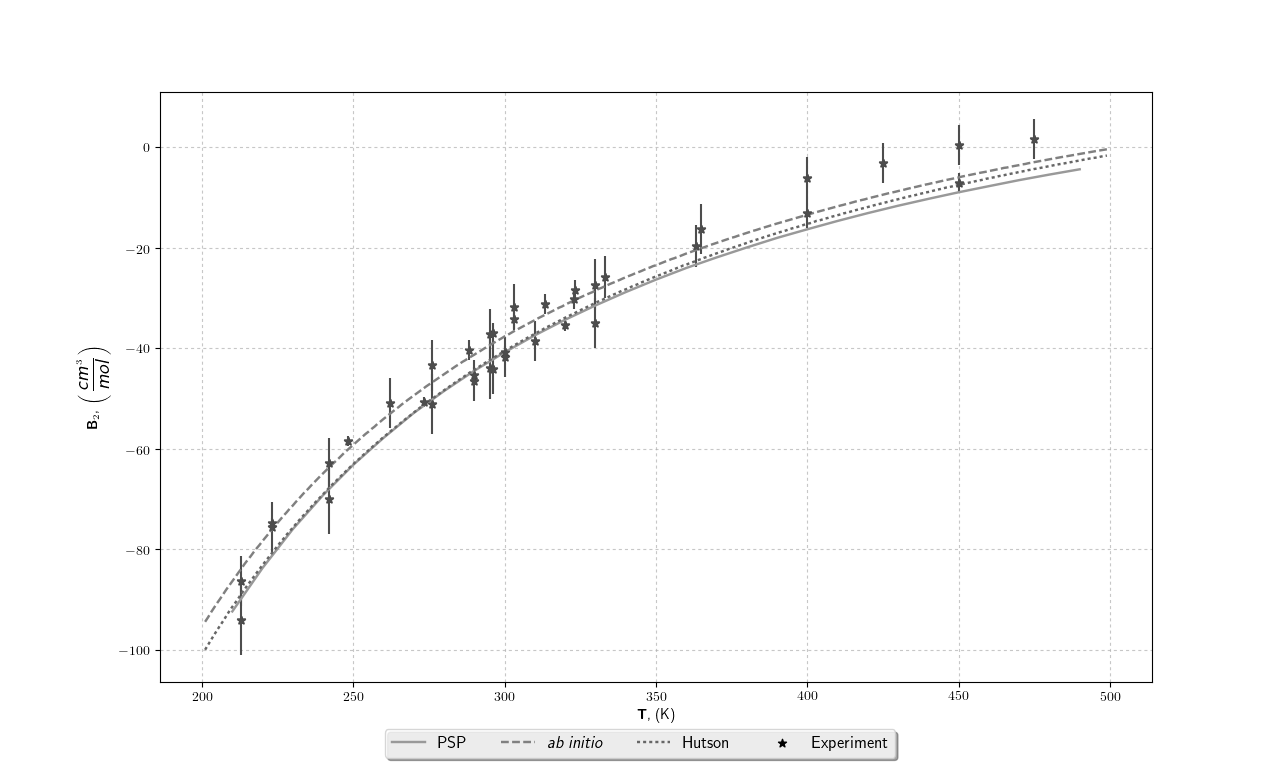
\includegraphics[width=\linewidth]{pictures/virexp.png}
\caption{Температурные зависимости вириальных коэффициентов для разных поверхностей потенциальной энергии. }
\label{fig:vir}
\end{figure}

\subsection{Квантовые поправки ко второму вириальному коэффициенту}

Термодинамические свойства ансамбля частиц могут быть рассчитаны с использованием суммы по состояниям
\vverh
\begin{gather}
	\sigma = \sum_n \exp \lb - \beta E_n \rb. \label{sigma}  
\end{gather}
Если устремить постоянную Планка $h$ к нулю, то сумма по состояниям \eqref{sigma} может быть преобразована в интеграл по фазовому пространству ансамбля:
\vverh
\begin{gather}
	\lim_{h \rightarrow 0} h^N \sigma = Z = \iint \exp \lb - \beta H(\mf{q}, \mf{p}) \rb d \mf{q} \, d \mf{p}, \label{sigma2}
\end{gather}
где $H(\mf{q}, \mf{p})$ -- классическая функция Гамильтона, а $N$ -- число степеней свободы системы. \par
Для квантовомеханических систем вычисление суммы по состояния \eqref{sigma} значительно более трудоемко. Для облегчения этой задачи была предложена процедура, позволяющая свести сумму по состояниям к интегралу по фазовому пространству, аналогичному Гиббсову интегралу \eqref{sigma2} \cite{kirkwood1933}. \par 
Рассмотрим ансамбль, состоящий из $N$ одинаковых частиц с массами $m$. Пусть потенциальная энергия системы $V \lb q_1, \dots q_{3N} \rb$  определяется только $3 N$ координатами частиц (положением фигуративной точки в конфигурационном пространстве ансамбля). Уравнение Шредингера такой системы 
\vverh
\begin{gather}
	\lb \hat{H} - E_n \rb \psi_n = 0, \quad \hat{H} = - \sum_{k = 1}^{N} \frac{\hbar^2}{2m} \Delta_k + V \lb q_1, \dots q_{3N} \rb, \notag 
\end{gather}
где $\psi_n$ -- нормированные волновые функции, соответствующие уровню $E_n$. Рассмотрим следующее выражение с оператором $\exp \lb - \beta \hat{H }\rb$:
\vverh
\begin{gather}
	\psi_n^{*} \exp \lb - \beta \hat{H} \rb \psi_n = \psi_n^{*} \sum_l \frac{ \lb - \beta \rb^l}{l!} \hat{H}^l \psi_n = \psi_n^{*} \sum_l \frac{ \lb - \beta \rb^l}{l!} E_n^l \psi_n = \psi_n^{*} \exp \lb - \beta E_n \rb \psi_n 
\end{gather}
Таким образом, сумма по состояниям \eqref{sigma} сводится к следующему интегралу по конфигурационному пространству:
\vverh
\begin{gather}
	\sigma = \sum_n \exp \lb - \beta E_n \rb = \sum_n \idotsint \psi_n^{*} \exp \lb - \beta H \rb \psi_n d q_1, \dots, d q_{3N}. \label{sigma3}  
\end{gather}

Конфигурационный интеграл \eqref{sigma3} может быть преобразован к фазовому интегралу, который оказывается существенно сложнее классического. Однако, для систем, проявляющих классические свойства, было показано, что такой интеграл может быть разложен в виде ряда по степеням постоянной Планка $h$, причем первым членом этого разложения является Гиббсов интеграл \eqref{sigma2} \cite{wigner1932, kirkwood1933}.

Аналогичное разложение второго вириального коэффициента по степеням постоянной Планка $h$ получило название разложения Вигнера-Кирквуда \cite{kirkwood1933} (т.к. первым членом в разложении суммы по состояниям $\sigma$ является классический фазовый интеграл, то первым членом в разложении вириального коэффициента является классический вириальный коэффициент). Оказалось, что в ряд входят только те слагаемые, которые содержат $h^2$. Разложение Вигнера-Кирквуда имеет вид (трансляционная и вращательная поправки обозначаются индексами $t$ и $r$ соотвественно)
\vverh
\begin{gather}
	B = B_{\text{класс.}} + \frac{\hbar^2}{m} B_{t1} + \lb \frac{\hbar^2}{m} \rb^2 B_{t2} + \dots + \frac{\hbar^2}{I} B_{r1} + \lb \frac{\hbar^2}{I} \rb^2 B_{r2} + \dots .\notag
\end{gather}

Строго разложение применимо только к линейным молекулам, т.к. содержит только один момент инерции. Поправки в разложении Вигнера-Кирквуда имеют вид (для потенциала $U = U(r, \theta_1, \theta_2, \phi_2 - \phi_1)$) \cite{meyson, hirsch} 
\vverh
\begin{gather}
	B_{t1} = \frac{N_0}{48 \lb kT \rb^3} \int\limits_{0}^{\infty} \int\limits_{\lb \Omega \rb} \exp \lb -\frac{U}{k T} \rb \lb \frac{\partial U}{\partial r} \rb^2 r^2 d r d \Omega, \notag \\
	B_{r1} = \frac{N_0}{96 \lb kT \rb^3} \int\limits_{0}^{\infty} \int\limits_{\lb \Omega \rb} \exp \lb -\frac{U}{k T} \rb \left[ \lb \frac{\partial U}{\partial \theta_1} \rb^2 + \lb \frac{\partial U}{\partial \theta_2} \rb^2 + \frac{1}{\sin^2 \theta_1} \lb \frac{\partial U}{\partial \phi_1} \rb^2 + \frac{1}{\sin^2 \theta_2} \lb \frac{\partial U}{\partial \phi_2} \rb^2 \right] r^2 d r d \Omega, \notag 
\end{gather}
где
\begin{gather}
	\int\limits_{\lb \Omega \rb} d \Omega = \int\limits_0^\pi \sin \theta_1 d \theta_1 \int\limits_0^\pi \sin \theta_2 d \theta_2 \int\limits_0^{2 \pi} d \lb \phi_2 - \phi_1 \rb. \notag
\end{gather}

Применительно к системе $Ar-CO_2$ получаем следующие выражения для квантовых поправок:
\vverh
\begin{gather}
	B_{t1} = \frac{\pi N_0}{12 \lb k T \rb^3} \int\limits_0^\infty \int\limits_0^\pi \exp \lb - \frac{U}{k T} \rb \lb \frac{\partial U}{\partial r} \rb^2 r^2 \sin \theta d r d \theta, \label{transcorr} \\
	B_{r1} = \frac{\pi N_0}{24 \lb k T \rb^3} \int\limits_0^\infty \int\limits_0^\pi \exp \lb - \frac{U}{k T} \rb \lb \frac{\partial U}{\partial \theta} \rb^2 r^2 \sin \theta d r d \theta. \label{rotcorr}
\end{gather}

Учитывая только квантовые поправки первого порядка вириальный коэффициент вычисляется следующим образом 
\vverh
\begin{gather}
	B = B_{\text{класс.}} + \frac{\hbar^2}{m} B_{t1} + \frac{\hbar^2}{I} B_{r1} = B^{(0)} + B_{tr}^{(1)} + B_{rot}^{(1)}. \notag
\end{gather}

В таблице $\lb \ref{tab:tablevir} \rb$ представлены значения квантовых поправок для системы $Ar-CO_2$, рассчитанные с \textit{ab-initio} потенциалом. Производные $\ddfrac{\strut\partial U}{\strut\partial r}$, $\ddfrac{\strut\partial U}{\strut\partial \theta}$, входящие в подынтгеральные выражения \eqref{transcorr} и \eqref{rotcorr} соответственно, были вычислены аналитически. Интегрирование производилось при помощи адаптивного метода Монте-Карло. (В первом столбце представлены значения вириальных коэффициентов, рассчитанные по классической формуле \eqref{virint}, во втором и третьем стобцах -- квантовые поправки, полученные по формулам \eqref{transcorr}, \eqref{rotcorr} соответственно, затем посчитано значение вириального коэффициента с учетом поправок, в последнем стобце представлено экспериментальное значение вириального коэффициента с ссылкой на публикацию). 

\newpage
\setlength{\tabcolsep}{12pt}
\begin{minipage}{\linewidth}
\centering
\vspace*{-0.5cm}

\captionof{table}{\centering Квантовые поправки для вириального коэффициента системы $Ar-CO_2$.} \label{tab:tablevir}
\vspace*{-0.3cm}
\fontsize{10pt}{12pt}\selectfont
\begin{tabular}{ccccccc}
\hline
\hline\noalign{\smallskip}
$T(K)$ & $B^{(0)}$ & $B_{tr}^{(1)}$ & $B_{rot}^{(1)}$ & $B$ & $B_{exp}$ \\
\noalign{\smallskip} \hline \noalign{\smallskip}
$213.$0 & $-83.79$ & $0.72$ & $0.14$ & $-82.93$ & \left\{ \hspace*{-3mm} \begin{tabular}{c} $-86.3 \pm 5.0^{\scriptsize \textbf{a}}$ \\ $-94.0 \pm 7.0^{\scriptsize \textbf{b}}$ \end{tabular} \right. \\
\noalign{\smallskip}

$223.0$ & $-76.09$ & $0.65$ & $0.13$ & $-75.13$ & \hspace*{-3mm} $-75.5 \pm 5.0^{\scriptsize \textbf{a}}$ \\
$233.0$ & & & & & \hspace*{-3mm} $-74.8 \pm 1.0^{\scriptsize \textbf{c}}$ \\
$242.0$ & $-63.68$ & $0.54$ & $0.11$ & $-63.03$ & \left\{ \hspace*{-3mm} \begin{tabular}{c} $-62.9 \pm 5.0^{\scriptsize \textbf{a}}$ \\ $-70.0 \pm 7.0^{\scriptsize \textbf{b}}$ \end{tabular} \right. \\
\noalign{\smallskip}

$248.2$ & $-60.16$ & $0.51$ & $0.10$ & $-59.55$ & \hspace*{-3mm} $-58.4 \pm 1.0^{\scriptsize \textbf{c}}$ \\
$262.0$ & $-53.06$ & $0.45$ & $0.09$ & $-52.52$ & \hspace*{-3mm} $-50.8 \pm 5.0^{\scriptsize \textbf{a}}$ \\
$273.2$ & $-47.96$ & $0.41$ & $0.08$ & $-47.47$ & \hspace*{-3mm} $-50.6 \pm 1.0^{\scriptsize \textbf{c}}$ \\
$276.0$ & $-46.75$ & $0.40$ & $0.08$ & $-46.27$ &  \left\{ \hspace*{-3mm} \begin{tabular}{c} $-43.4 \pm 5.0^{\scriptsize \textbf{a}}$ \\ $-51.0 \pm 6.0^{\scriptsize \textbf{b}}$ \end{tabular} \\
\noalign{\smallskip}

$288.2$ & $-41.89$ & $0.37$ & $0.07$ & $-41.45$ & \hspace*{-3mm} $-40.3 \pm 2.0^{\scriptsize \textbf{d}}$ \\
$290.0$ & $-41.21$ & $0.36$ & $0.07$ & $-40.78$ & \left\{ \hspace*{-3mm} \begin{tabular}{c} $-45.2 \pm 1.4^{\scriptsize \textbf{e}}$ \\ $-46.4 \pm 4.0^{\scriptsize \textbf{f}}$ \end{tabular} \right. \\
\noalign{\smallskip}

$295.0$ & $-39.37$ & $0.35$ & $0.07$ & $-38.95$ & \left\{ \hspace*{-3mm} \begin{tabular}{c} $-37.2 \pm 5.0^{\scriptsize \textbf{a}}$ \\ $-44.0 \pm 6.0^{\scriptsize \textbf{b}}$ \end{tabular} \right. \\
\noalign{\smallskip}

$296.0$ & $-39.02$ & $0.35$ & $0.07$ & $-38.60$ & \hspace*{-3mm} $-37.0 \pm 2.0^{\scriptsize \textbf{d}}$ \\
$296.15$ & $-38.97$ & $0.35$ & $0.07$ & $-38.55$ & \hspace*{-3mm} $-44.1 \pm 5.0^{\scriptsize \textbf{b}}$ \\
$300.0$ & $-37.63$ & $0.34$ & $0.07$ & $-37.22$ & \left\{ \hspace*{-3mm} \begin{tabular}{c} $-40.8 \pm 1.3^{\scriptsize \textbf{e}}$ \\ $-41.7 \pm 4.0^{\scriptsize \textbf{f}}$ \end{tabular} \right. \\
\noalign{\smallskip}

$303.15$ & $-36.55$ & $0.33$ & $0.06$ & $-36.16$ & \hspace*{-3mm} $-31.8 \pm 4.6^{\scriptsize \textbf{g}}$ \\
$303.2$ & $-36.55$ & $0.33$ & $0.06$ & $-36.16$ & \hspace*{-3mm} $-34.2 \pm 2.0^{\scriptsize \textbf{d}}$ \\
$310.0$ & $-34.34$ & $0.32$ & $0.06$ & $-33.96$ & \hspace*{-3mm} $-38.6 \pm 4.0^{\scriptsize \textbf{f}}$ \\
$313.2$ & $-33.34$ & $0.31$ & $0.06$ & $-32.97$ & \hspace*{-3mm} $-31.2 \pm 2.0^{\scriptsize \textbf{d}}$ \\
$320.0$ & $-31.30$ & $0.30$ & $0.06$ & $-30.94$ & \hspace*{-3mm} $-35.3 \pm 1.3^{\scriptsize \textbf{e}}$ \\
$322.85$ & $-30.48$ & $0.29$ & $0.06$ & $-30.13$ & \hspace*{-3mm} $-30.1 \pm 2.0^{\scriptsize \textbf{h}}$ \\
$323.1$ & $-30.40$ & $0.29$ & $0.06$ & $-30.05$ & \hspace*{-3mm} $-28.3 \pm 2.0^{\scriptsize \textbf{d}}$ \\
$330.0$ & $-28.48$ & $0.28$ & $0.05$ & $-28.15$ & \left\{ \hspace*{-3mm} \begin{tabular}{c} $-27.3 \pm 5.0^{\scriptsize \textbf{a}}$ \\ $-35.0 \pm 5.0^{\scriptsize \textbf{b}}$ \end{tabular} \right. \\
\noalign{\smallskip}

$333.15$ & $-27.63$ & $0.27$ & $0.05$ & $-27.95$ & \hspace*{-3mm} $-25.8 \pm 4.2^{\scriptsize \textbf{g}}$ \\
$363.15$ & $-20.46$ & $0.23$ & $0.04$ & $-20.19$ & \hspace*{-3mm} $-19.6 \pm 4.2^{\scriptsize \textbf{g}}$ \\
$365.0$ & $-20.06$ & $0.23$ & $0.04$ & $-19.79$ & \hspace*{-3mm} $-16.2 \pm 5.0^{\scriptsize \textbf{a}}$ \\
$400.0$ & $-13.39$ & $0.19$ & $0.04$ & $-13.16$ & \left\{ \hspace*{-3mm} \begin{tabular}{c} $-6.0 \pm 4.0^{\scriptsize \textbf{a}}$ \\ $-13.0 \pm 3.0^{\scriptsize \textbf{b}}$ \end{tabular} \right. \\
\noalign{\smallskip}

$425.0$ & $-9.42$ & $0.17$ & $0.03$ & $-9.22$ & \hspace*{-2mm} $-3.1 \pm 4.0^{\scriptsize \textbf{a}}$ \\
$450.0$ & $-5.97$ & $0.16$ & $0.03$ & $-5.78$ & \left\{ \hspace*{-2mm} \begin{tabular}{c} $0.5 \pm 4.0^{\scriptsize \textbf{a}}$ \\ $-7.0 \pm 2.0^{\scriptsize \textbf{b}}$ \end{tabular} \right. \\
\noalign{\smallskip}

$475.0$ & $-2.94$ & $0.14$ & $0.03$ & $-2.77$ & \hspace*{-1mm} $1.7 \pm 4.0^{\scriptsize \textbf{a}}$ \\ 
\noalign{\smallskip} \hline \hline
\end{tabular} \par
{\scriptsize
\begin{flushleft}
${}^{\scriptsize \textbf{a}}$Schmiedel, H.; Gehrmann, R.; Schramm, B.; Ber. Bunsen-Gest. Phys. Chem. \textbf{84} (1980) 721. \\
${}^{\scriptsize \textbf{b}}$Schramm, B.; Mueller, W.; Ber. Bunsen-Ges. Phys. Chem. \textbf{86} (1982) 110. \\
${}^{\scriptsize \textbf{c}}$Brewer, J.; Air Force Off.Sci. Res., [Tech. Rep.] AFOSR-TR 67-2795, (1967). \\
${}^{\scriptsize \textbf{d}}$Lichtenthaler, R. N.; Schaefer, K.; Ber. Bunsen-Ges. Phys. Chem. \textbf{73} (1969) 42. \\
${}^{\scriptsize \textbf{e}}$Martin, M.L.; Trengove, R.D.; Harris, J.R.; Dunlop, P.J.; Aust. J. Chem. \textbf{35} (1982) 1525. \\
${}^{\scriptsize \textbf{f}}$Bell, T. N.; Bignell, C.M.l Dunlop, P.J.; Physica A: (Amsterdam) \textbf{181} (1992) 221. \\
${}^{\scriptsize \textbf{g}}$Cottrell, T.L.; Hamilton R. A.; Taubinger, R.P.; Trans. Faraday Soc. \textbf{52} (1956) 1310. \\
${}^{\scriptsize \textbf{h}}$Bose, T.K.; Cole, R.H.; J. Chem. Phys. \textbf{52} (1970) 140.
\end{flushleft}
}
\end{minipage}

